\chapter{Definição da Interface com o Usuário}

A interface do \textit{Civitas} organiza as tarefas administrativas e financeiras descritas nos capítulos anteriores em fluxos compreensíveis para os perfis Administrador, Funcionário e Visitante. O projeto de interação considera o objetivo de cada tarefa, os dados necessários para concluí-la e a resposta que o sistema deve apresentar. Cenários, personas, esboços e protótipos permitem examinar a experiência antes e durante a implementação \parencite{Rogers2013,Garrett2011}. As representações desta seção correspondem aos requisitos funcionais do Quadro~\ref{quad:requisitos_funcionais} e aos atores da Seção~\ref{sec:definicao-atores-civitas-final}.

\section{Descrição de Cenário}

Um cenário descreve, em forma de narrativa, o contexto, a intenção e as ações de uma pessoa ao utilizar um sistema. Essa forma de representação torna visíveis as decisões exigidas pela tarefa e ajuda a conferir se a interface oferece informações e respostas suficientes em cada etapa \parencite{Rogers2013}. Os dois cenários a seguir foram escolhidos por envolverem, respectivamente, o registro operacional de uma despesa e o acompanhamento administrativo dos dados consolidados. Os nomes e a situação concreta são ilustrativos; as operações correspondem aos requisitos e aos casos de uso documentados para o \textit{Civitas}.

O primeiro cenário, apresentado no Quadro~\ref{qua:cap4-despesa}, concentra a relação entre a despesa e a unidade consumidora. Essa relação importa porque o fornecedor, a instituição, o tipo de despesa e o orçamento são alcançados por meio da unidade selecionada, conforme RF10 e RF11. Também permite examinar como o formulário informa campos obrigatórios e erros antes de concluir o lançamento.

\begin{quadro}[H]
\caption{Cenário -- Registro de despesa municipal}\label{qua:cap4-despesa}
\begin{tabularx}{\textwidth}{@{}X@{}}
\toprule
Rafael, funcionário do setor financeiro, recebe um documento referente ao consumo de uma unidade vinculada a uma instituição municipal. Após entrar no \textit{Civitas}, consulta a relação de despesas para verificar se o número do documento já consta entre os lançamentos. Ao iniciar um novo registro, seleciona a unidade consumidora pertinente e confere os vínculos apresentados para instituição, fornecedor, tipo de despesa e orçamento. Em seguida, informa o número do documento, as datas de emissão e vencimento, os valores e o consumo previstos e associa o arquivo comprobatório solicitado pelo formulário. Se algum dado obrigatório estiver ausente ou inconsistente, corrige-o a partir da mensagem exibida. Depois da confirmação, retorna à listagem para localizar a despesa e acompanhar sua condição financeira.\\
\bottomrule
\end{tabularx}
\fonte{Elaborado pelos autores.}
\end{quadro}

O resultado esperado é um lançamento consultável, associado à unidade consumidora e ao usuário responsável. O cenário não pressupõe aprovação automática, notificação externa ou pagamento no momento do cadastro. O pagamento constitui uma etapa própria, representada no sistema por campos e ações específicos de baixa e comprovante, conforme RF12.

O segundo cenário (Quadro~\ref{qua:cap4-painel}) representa uma atividade de supervisão do Administrador. Ele verifica se os indicadores sintetizam os lançamentos e se oferecem caminhos claros para consultar os registros que exigem análise, em correspondência com RF14 e RF15.

\begin{quadro}[H]
\caption{Cenário -- Acompanhamento financeiro no painel}\label{qua:cap4-painel}
\begin{tabularx}{\textwidth}{@{}X@{}}
\toprule
Helena, administradora responsável por acompanhar os dados de gestão, entra no \textit{Civitas} para preparar uma conferência interna. No painel, observa o total orçado, o total gasto, o saldo e os quantitativos cadastrais. Utiliza a opção de exibir valores quando precisa examinar os montantes e verifica a relação de despesas recentes e os vencimentos próximos. Ao identificar um lançamento que necessita conferência, utiliza a pesquisa ou a navegação para abrir a área de despesas, aplica os filtros disponíveis e consulta o registro detalhado. A consulta permite relacionar o resumo apresentado no painel aos dados que o compõem, sem alterar o lançamento durante essa etapa.\\
\bottomrule
\end{tabularx}
\fonte{Elaborado pelos autores.}
\end{quadro}

Esse cenário evidencia a passagem da visão sintética à consulta detalhada. O painel oferece apoio à conferência, mas os indicadores não substituem a inspeção dos registros de origem nem constituem, por si, um procedimento de prestação de contas.

\section{Descrição de Personas}

\textit{Personas} são representações sintéticas de perfis de uso que ajudam a relacionar objetivos, tarefas e dificuldades às decisões de interface. Sua utilidade está em manter o foco nas necessidades de quem executa o trabalho, sem confundir um perfil projetual com uma pessoa real \parencite{Unger2012}. As duas personas deste capítulo são hipóteses de projeto construídas a partir dos atores, casos de uso e requisitos do \textit{Civitas}; nomes e idades são fictícios. Elas não são apresentadas como resultado de entrevistas ou de validação com servidores municipais.

A primeira persona (Figura~\ref{fig:cap4-persona-admin}) representa o Administrador, perfil ao qual o Capítulo 3 atribui gestão de usuários, cadastros estruturais, orçamentos e consulta de auditoria. A necessidade de conferir diferentes módulos orienta uma navegação consistente e a passagem rápida de indicadores para listagens detalhadas.

\begin{figure}[H]
\centering
\caption{Persona 1 -- Helena Martins, Administradora}
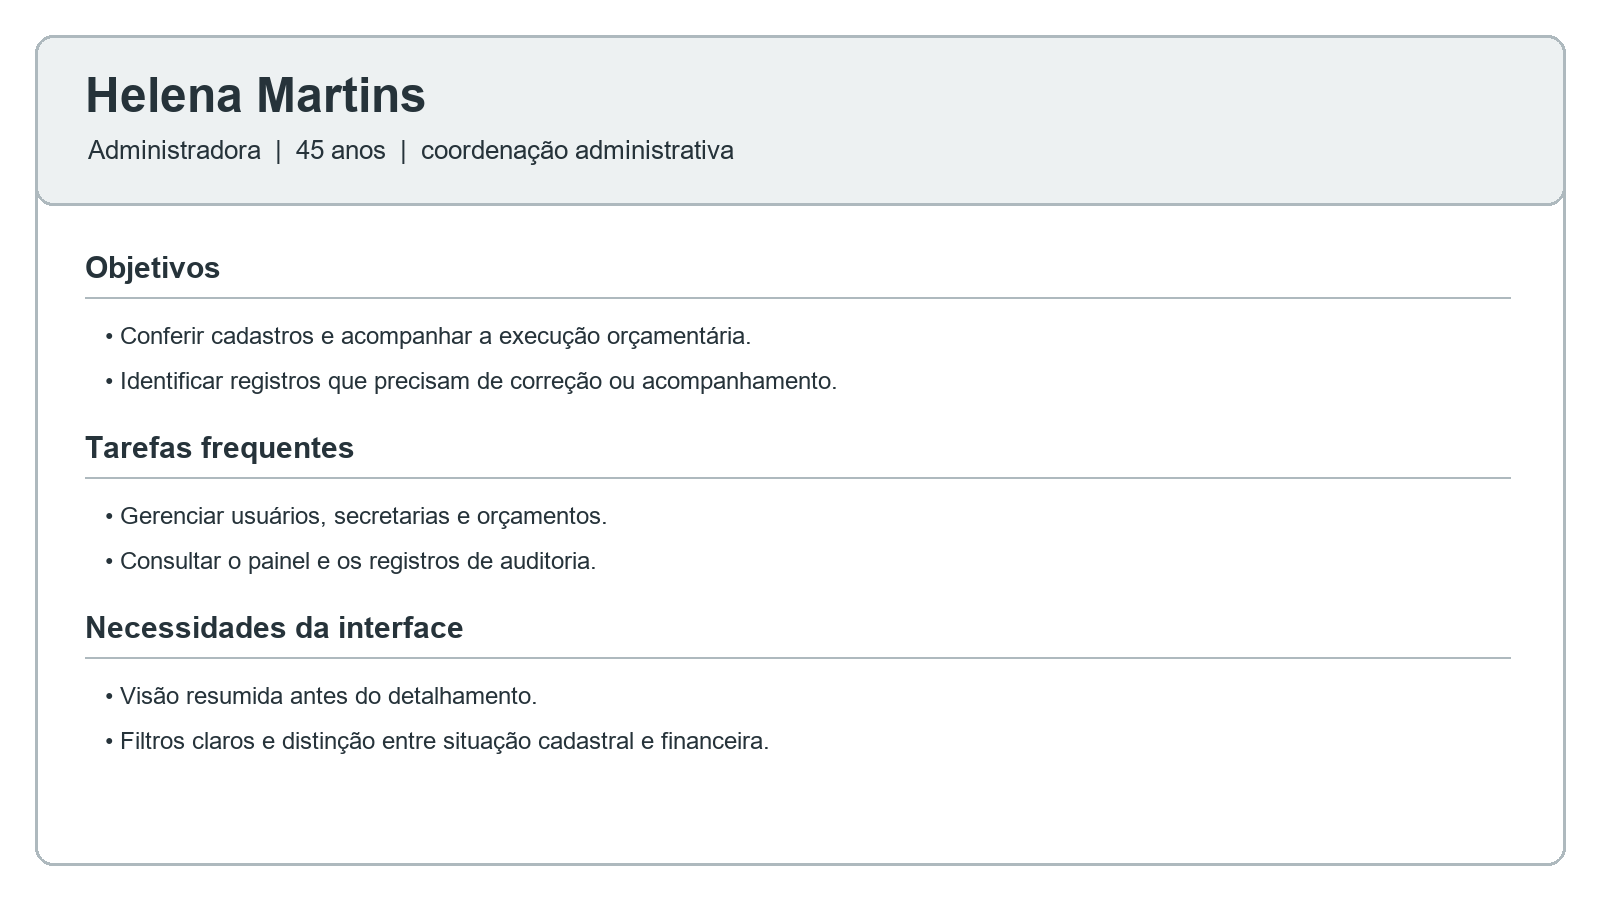
\includegraphics[width=.94\linewidth]{figs/cap4_persona_administradora.png}
\label{fig:cap4-persona-admin}
\fonte{Elaborada pelos autores.}
\end{figure}

Para Helena, o painel gerencial deve identificar os indicadores antes de apresentar as tabelas extensas. Nas páginas de usuários, secretarias e orçamentos, títulos, filtros e ações precisam indicar claramente qual conjunto de dados está em manutenção. A separação visual entre situação cadastral e condição financeira evita interpretar um registro inativo como uma despesa paga ou atrasada. A consulta de auditoria é pertinente a esse perfil, mas não deve aparecer como tarefa operacional do Funcionário.

A segunda persona (Figura~\ref{fig:cap4-persona-func}) representa o Funcionário que registra e consulta despesas. Seus casos de uso incluem consulta de orçamentos, manutenção de fornecedores e instituições, cadastro de despesas e consulta de documentos associados, sem gestão de usuários ou acesso aos registros de auditoria.

\begin{figure}[H]
\centering
\caption{Persona 2 -- Rafael Lima, Funcionário}
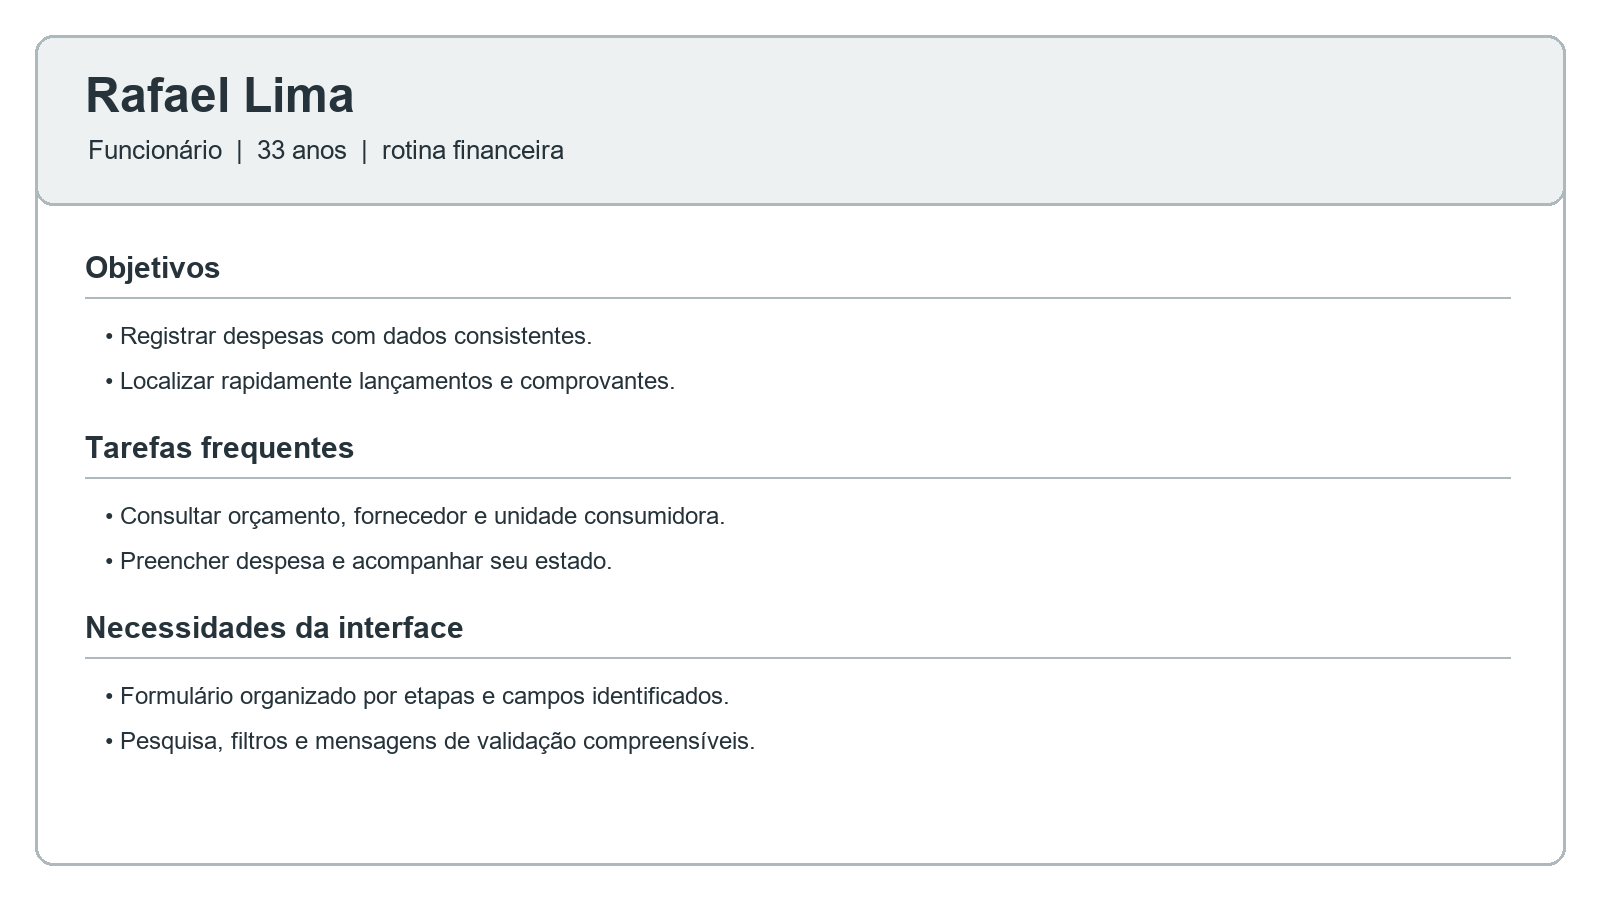
\includegraphics[width=.94\linewidth]{figs/cap4_persona_funcionario.png}
\label{fig:cap4-persona-func}
\fonte{Elaborada pelos autores.}
\end{figure}

Para Rafael, a interface precisa preservar a relação entre unidade consumidora e os dados financeiros que dela decorrem. A organização do formulário por grupos, os rótulos dos campos, a pesquisa e os filtros reduzem a necessidade de memorizar identificadores. Mensagens de validação devem indicar qual informação corrigir, e a listagem deve permitir verificar o resultado do lançamento. O Visitante permanece como ator consultivo na modelagem, sem constituir uma terceira persona operacional.

\section{Esboços de Tela (\textit{Wireframes})}

\textit{Wireframes} são representações de baixa fidelidade usadas para discutir a distribuição de conteúdo, a sequência de ações e a hierarquia da informação antes do acabamento visual. Ao omitir cores e dados reais, o esboço favorece a análise dos componentes e das relações entre as telas \parencite{Garrett2011,Buxton2007}. Os desenhos desta seção foram elaborados a partir dos fluxos e componentes identificados no frontend do \textit{Civitas}; não representam capturas de uma versão publicada nem resultados de teste com usuários.

A Figura~\ref{fig:cap4-wire-login} mostra o acesso ao ambiente interno. A apresentação institucional ocupa uma área separada do formulário, enquanto os campos de e-mail e senha, a opção \emph{Lembrar-me}, o caminho de recuperação de senha e a ação \emph{Entrar} seguem uma ordem única de leitura. Esse fluxo corresponde à autenticação prevista em RF01.

\begin{figure}[H]
\centering
\caption{Wireframe -- Tela de login do Civitas}
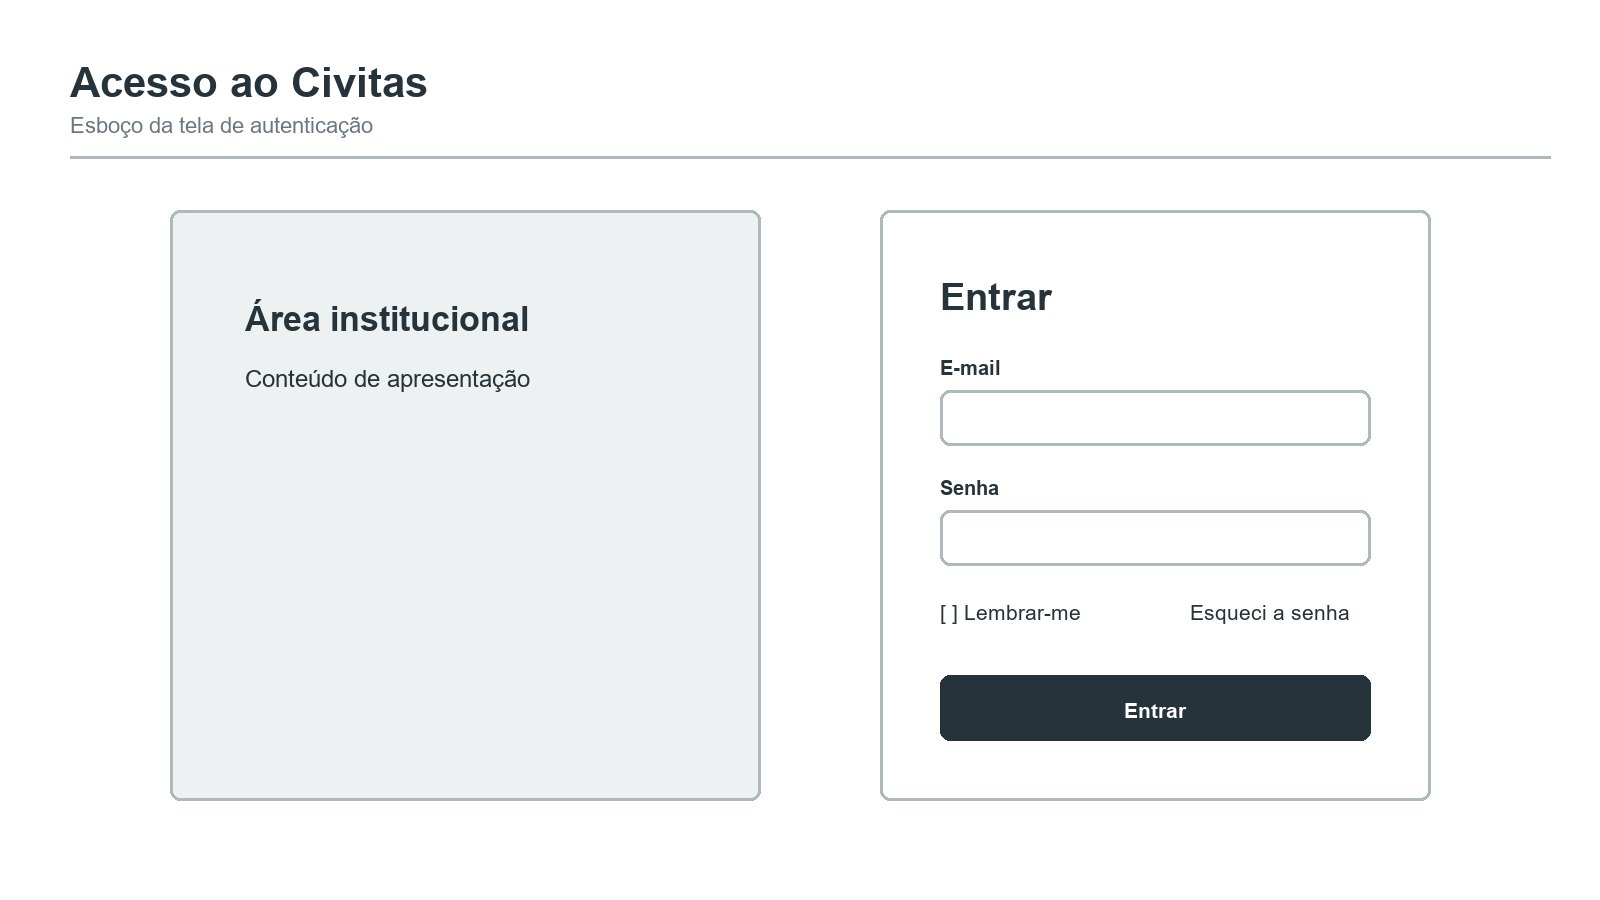
\includegraphics[width=.94\linewidth]{figs/cap4_wireframe_login.png}
\label{fig:cap4-wire-login}
\fonte{Elaborada pelos autores.}
\end{figure}

O painel da Figura~\ref{fig:cap4-wire-painel} prioriza os valores consolidados, seguidos da pesquisa e da relação de despesas recentes. A barra lateral situa o usuário entre as áreas principais e os cartões permitem leitura rápida antes do exame de registros específicos. Os dados desenhados são apenas marcadores de posição, sem valores financeiros fictícios.

\begin{figure}[H]
\centering
\caption{Wireframe -- Painel gerencial do Civitas}
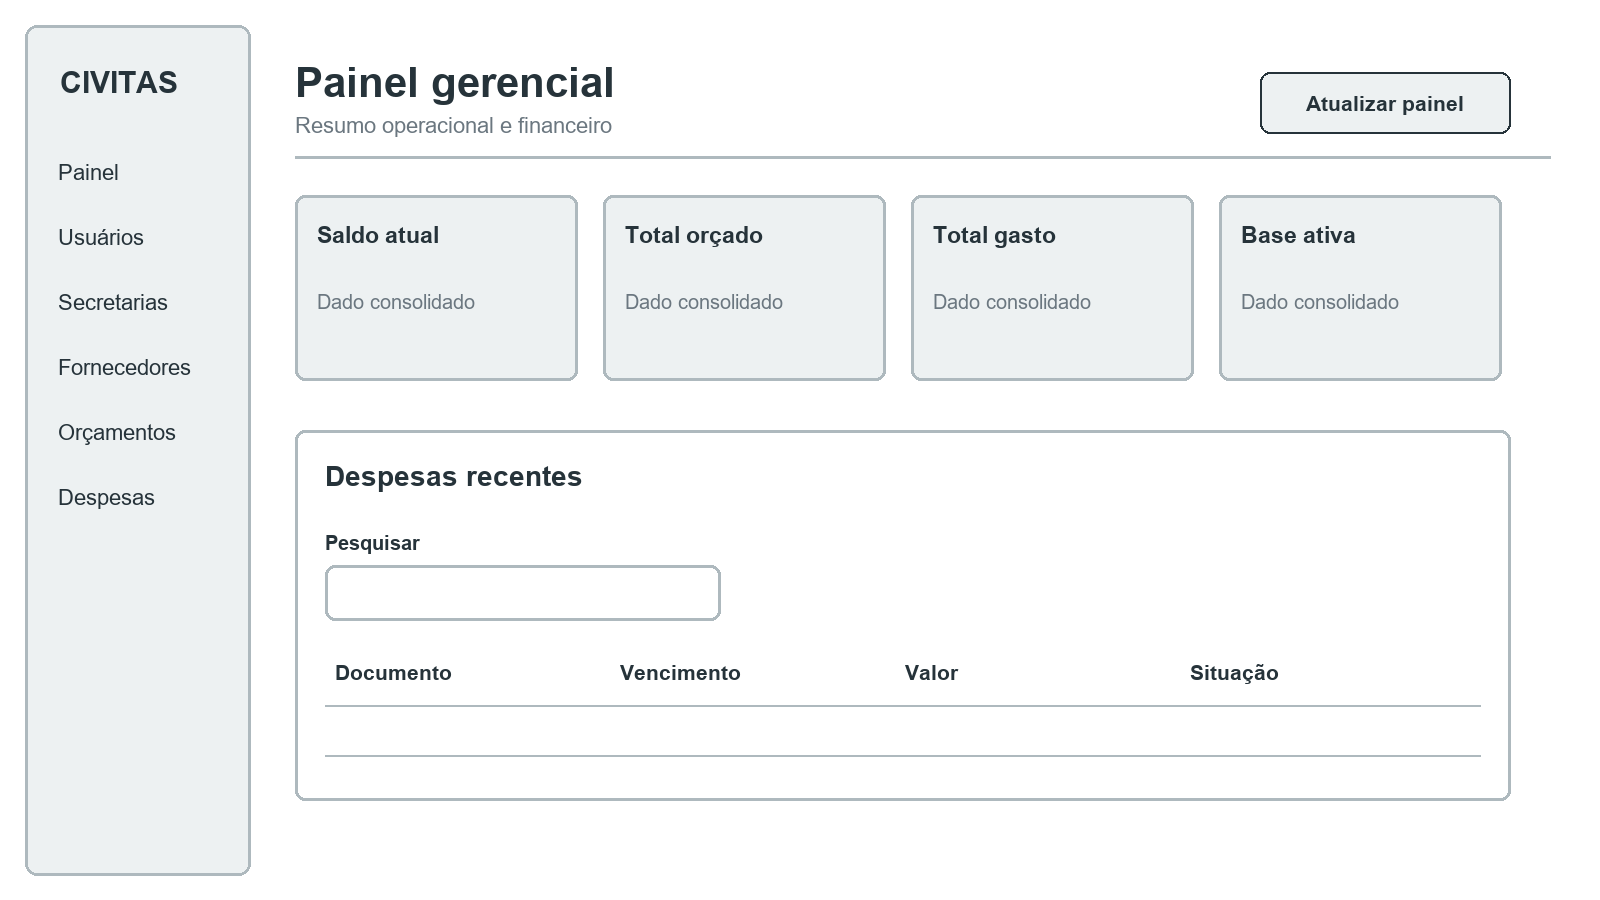
\includegraphics[width=.94\linewidth]{figs/cap4_wireframe_painel.png}
\label{fig:cap4-wire-painel}
\fonte{Elaborada pelos autores.}
\end{figure}

A Figura~\ref{fig:cap4-wire-usuarios} documenta uma operação administrativa do perfil Administrador: localizar contas, consultar seus atributos e iniciar um cadastro. O filtro fica antes da tabela, enquanto a ação de inclusão ocupa posição destacada. Essa organização permite distinguir a busca de um usuário existente da criação de uma conta, em consonância com RF03 e RF04.

\begin{figure}[H]
\centering
\caption{Wireframe -- Gestão de usuários do Civitas}
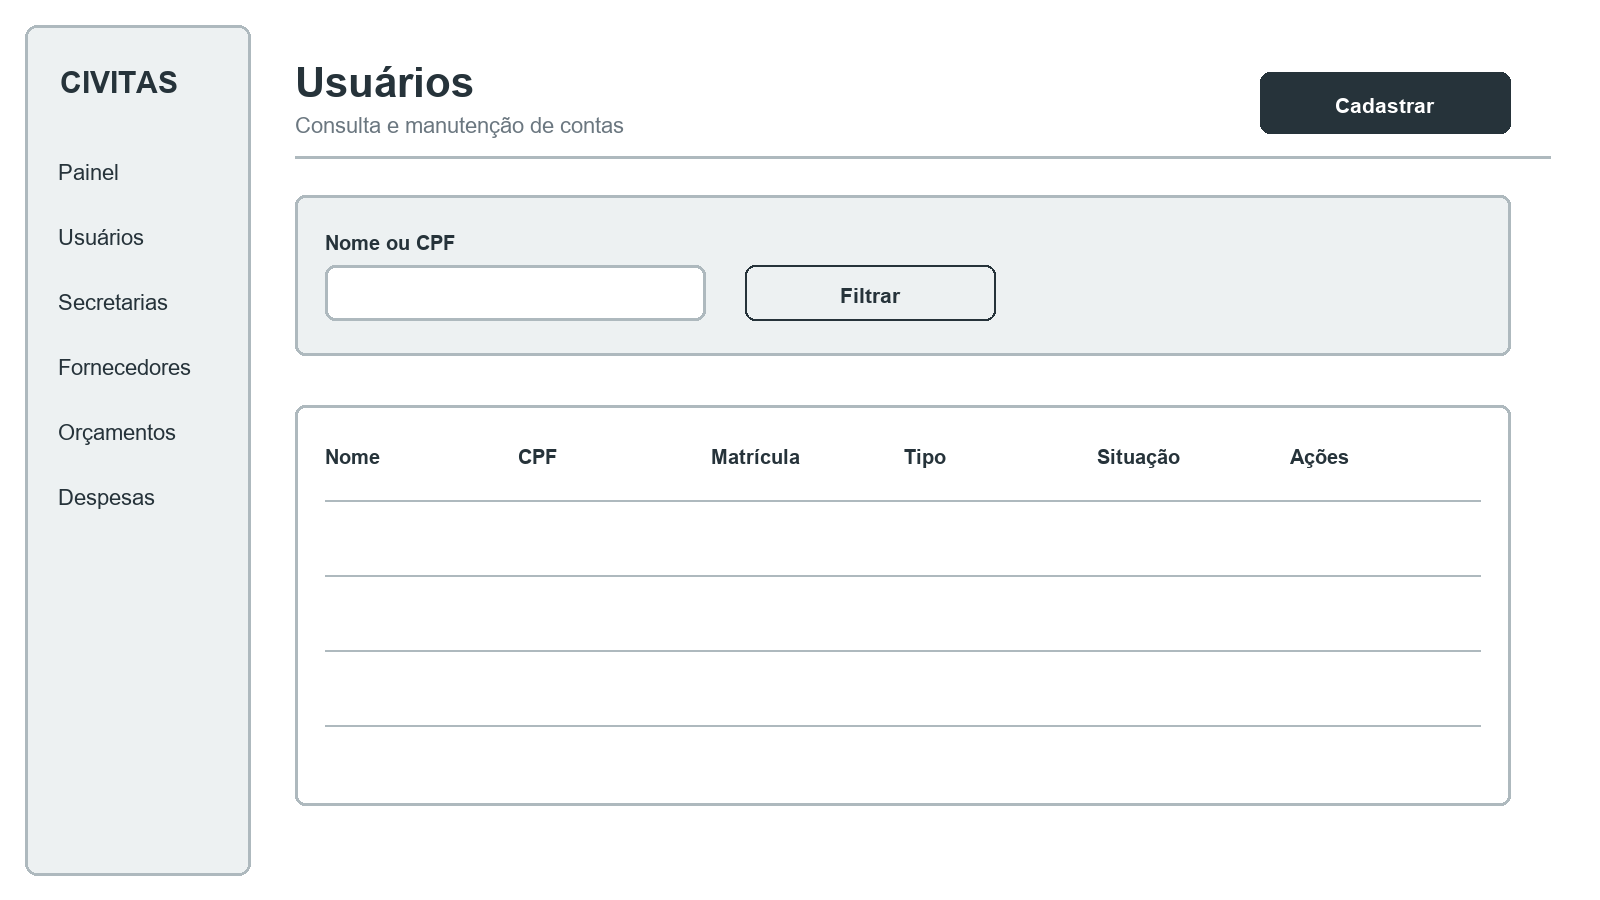
\includegraphics[width=.94\linewidth]{figs/cap4_wireframe_usuarios.png}
\label{fig:cap4-wire-usuarios}
\fonte{Elaborada pelos autores.}
\end{figure}

Na Figura~\ref{fig:cap4-wire-despesas}, a tarefa financeira começa pela localização dos lançamentos com busca, período e instituição; a ação de nova despesa inicia o formulário. As colunas reservam espaço para documento, instituição, vencimento, valor, estado e ações contextuais. O esboço evidencia a diferença entre consultar uma despesa e registrar outra, sem sugerir que a listagem seja uma planilha de edição direta.

\begin{figure}[H]
\centering
\caption{Wireframe -- Listagem de despesas do Civitas}
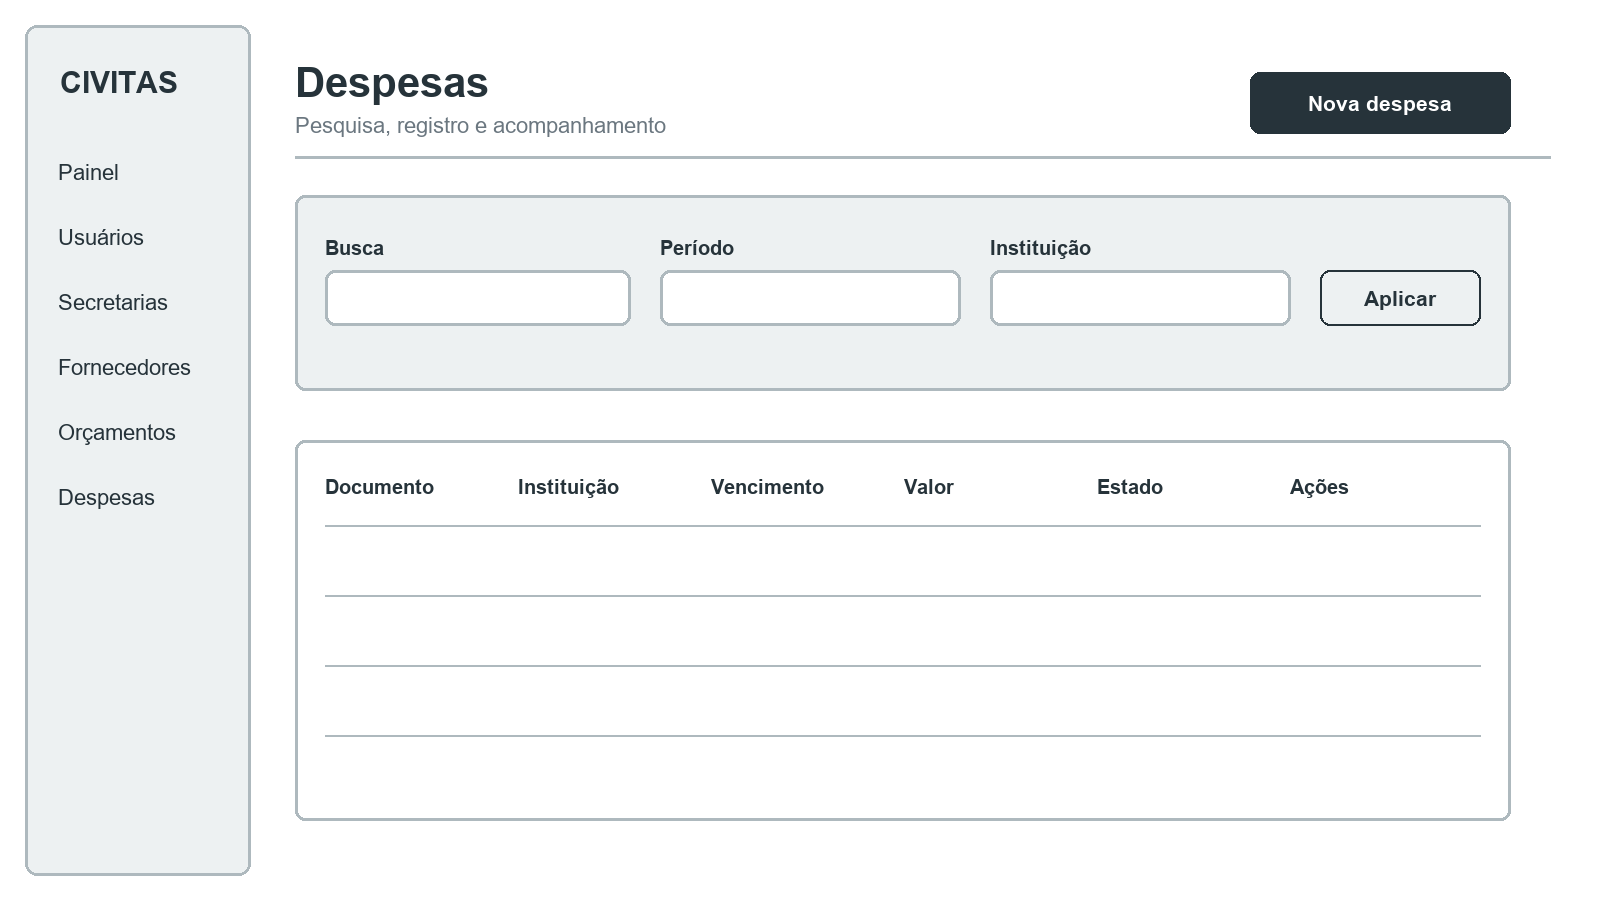
\includegraphics[width=.94\linewidth]{figs/cap4_wireframe_despesas.png}
\label{fig:cap4-wire-despesas}
\fonte{Elaborada pelos autores.}
\end{figure}

\section{Protótipos de Tela}

Protótipos com maior fidelidade acrescentam tipografia, cores, estados e componentes concretos aos fluxos definidos nos esboços. Eles permitem discutir a legibilidade e a coerência visual das soluções propostas, embora uma imagem estática não comprove, por si, o comportamento de todas as interações \parencite{Garrett2011,Buxton2007}. As Figuras~\ref{fig:cap4-proto-login}, \ref{fig:cap4-proto-secretarias} e \ref{fig:cap4-proto-despesas} provêm dos artefatos de sprint do frontend do \textit{Civitas}. São registros de versões de projeto e, por isso, os detalhes de texto e disposição podem diferir da implementação em evolução. As descrições abaixo se limitam aos elementos visíveis e aos fluxos que também aparecem no código atual.

A Figura~\ref{fig:cap4-proto-login}, registrada na tarefa de implementação do login, apresenta a marca, o formulário de e-mail e senha, a opção de lembrar o acesso, o caminho de recuperação e a ação principal. A captura documenta o estado de validação com mensagens textuais abaixo dos campos. O menu de acessibilidade aparece à direita, reunindo controles de tamanho da fonte e contraste. Essa composição concentra a atenção na autenticação e fornece retorno específico quando os campos estão vazios.

\begin{figure}[H]
\centering
\caption{Civitas -- Tela de login e mensagens de validação}
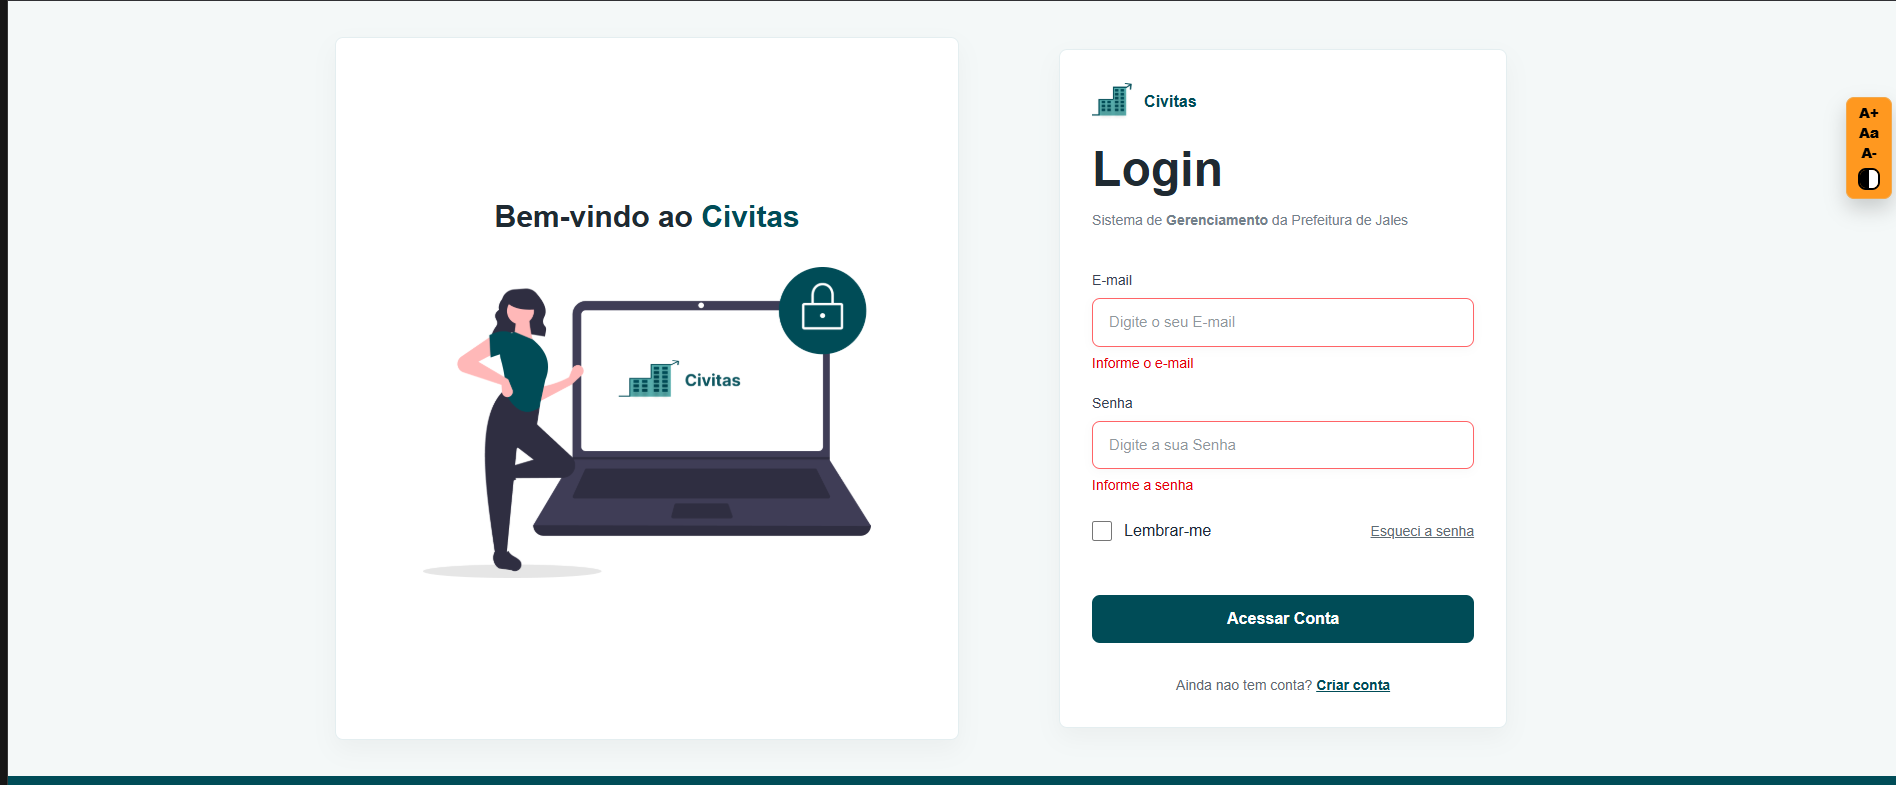
\includegraphics[width=.94\linewidth]{figs/cap4_tela_login_civitas.png}
\label{fig:cap4-proto-login}
\fonte{Documentação do frontend Civitas, tarefa Sprint 15 -- Login básico com persistência local.}
\end{figure}

O protótipo de secretarias da Figura~\ref{fig:cap4-proto-secretarias} mostra a navegação lateral, o título da página, campos de busca, filtros, ação de cadastro e listagem com situação e ações por registro. A tela corresponde à necessidade de consultar e manter secretarias em RF05. Os símbolos na coluna de ações representam opções de interação do protótipo; a regra de alteração de situação e as permissões efetivas devem seguir os casos de uso e a implementação.

\begin{figure}[H]
\centering
\caption{Civitas -- Protótipo de listagem de secretarias}
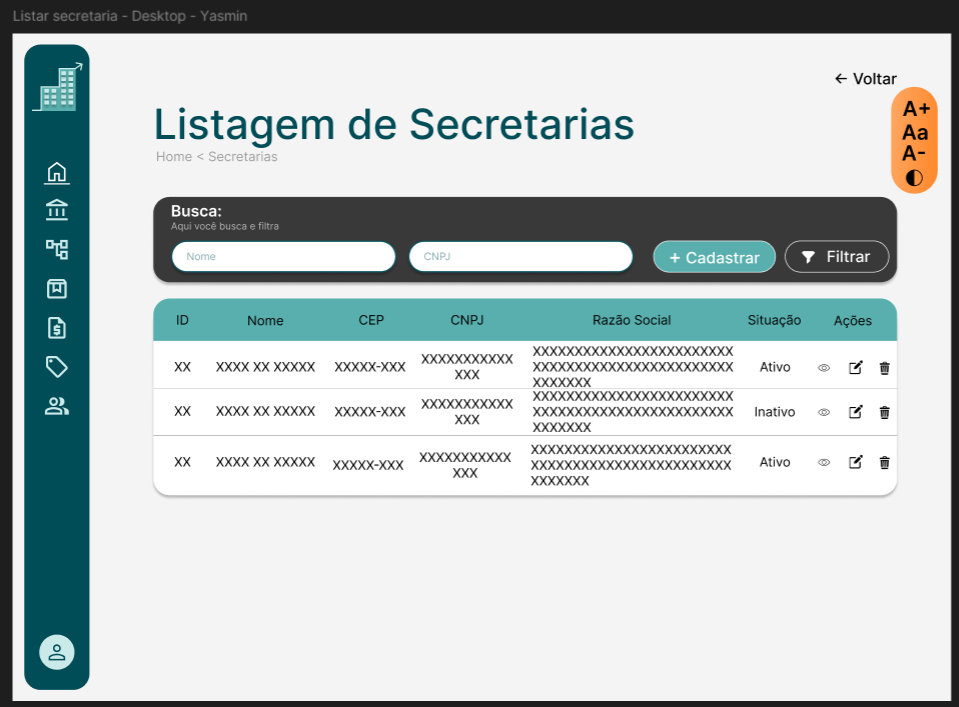
\includegraphics[width=.84\linewidth]{figs/cap4_prototipo_secretarias_civitas.png}
\label{fig:cap4-proto-secretarias}
\fonte{Documentação do frontend Civitas, tarefa Sprint 03 -- Protótipo de listagem de secretarias.}
\end{figure}

A Figura~\ref{fig:cap4-proto-despesas} registra um protótipo posterior de consulta de despesas. A ação de cadastro aparece antes dos cartões de saldo, entrada e saída; a área de filtros permite restringir o período e as características do lançamento; a tabela organiza os resultados e as ações de cada linha. A hierarquia conduz da visão geral ao conjunto filtrado e, por fim, ao registro específico. Os valores e lançamentos exibidos são exemplos do protótipo, não dados reais da administração municipal; a figura tampouco substitui a conferência da interface implementada.

\begin{figure}[H]
\centering
\caption{Civitas -- Protótipo de listagem de despesas}
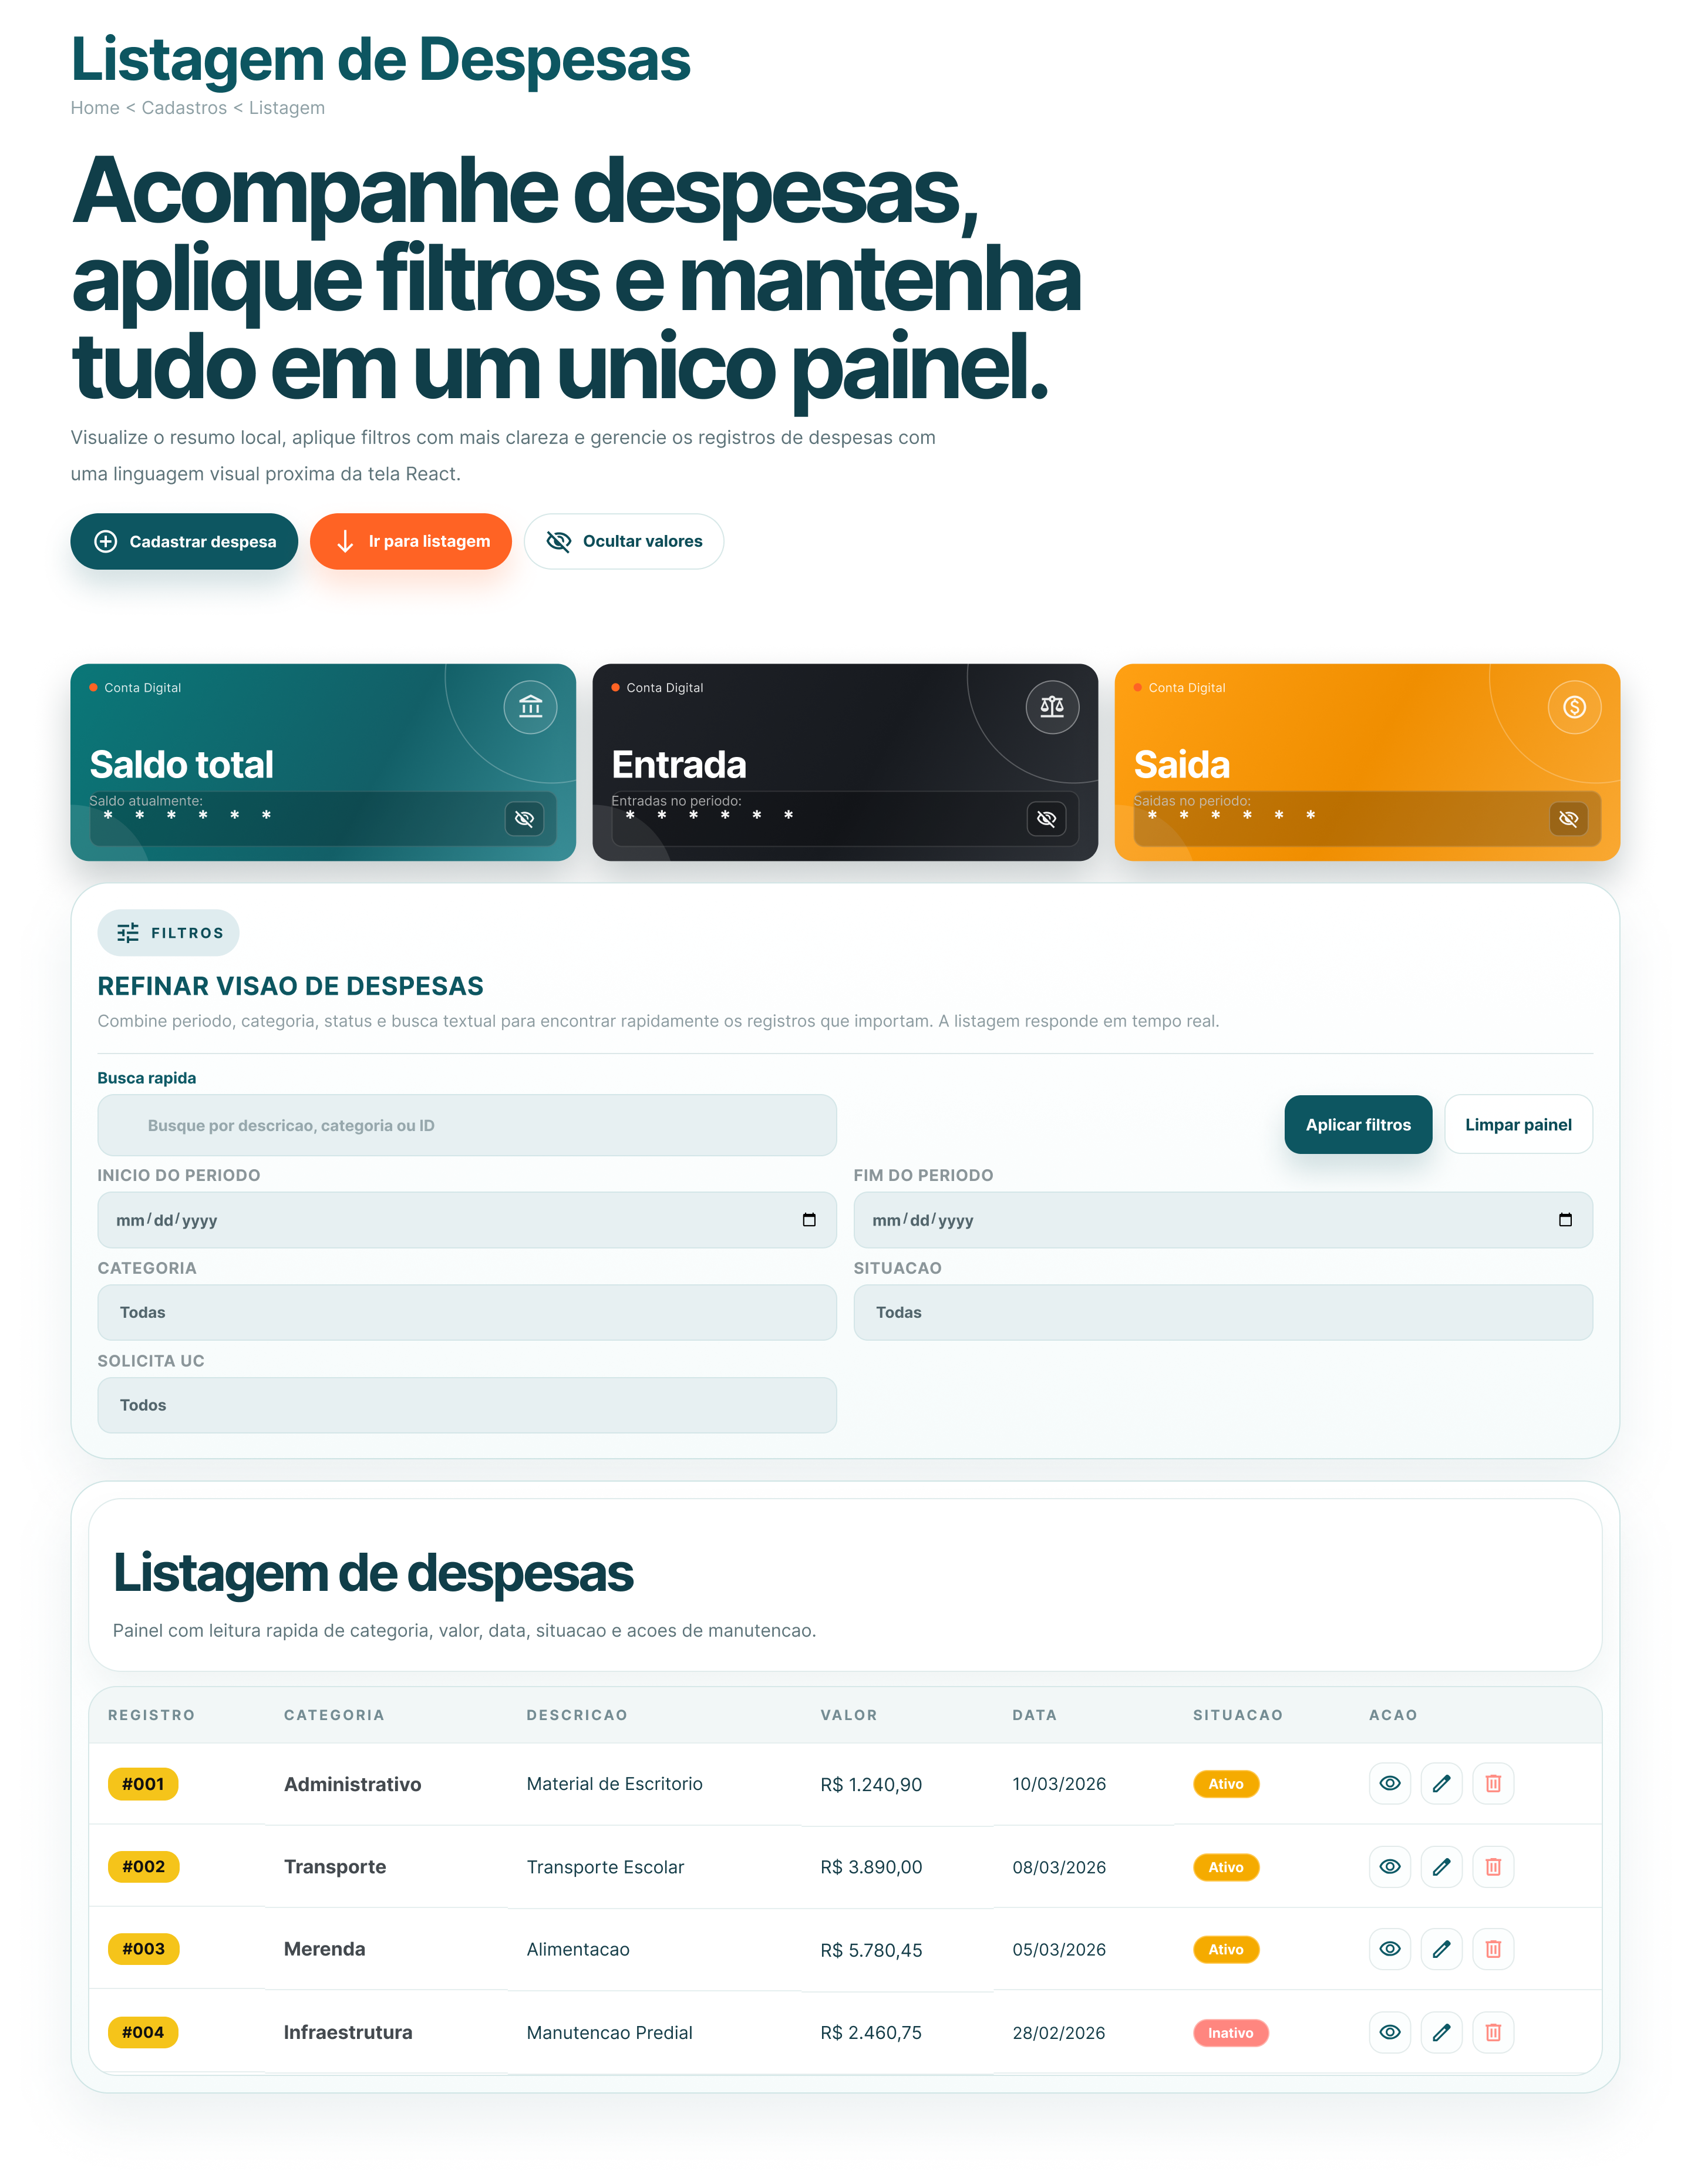
\includegraphics[width=.77\linewidth]{figs/cap4_prototipo_despesas_civitas.png}
\label{fig:cap4-proto-despesas}
\fonte{Documentação do frontend Civitas, tarefa Sprint 14 -- Protótipo da página de despesas.}
\end{figure}

\section{Acessibilidade e Inclusão de Pessoas com Deficiência}

A inclusão digital exige considerar as barreiras que podem surgir durante a percepção do conteúdo, a navegação e a execução de tarefas. A Convenção promulgada pelo Decreto nº 6.949/2009 trata da participação das pessoas com deficiência em igualdade de condições, enquanto a Lei Brasileira de Inclusão estabelece a acessibilidade como condição de uso seguro e autônomo de espaços, serviços, informação e comunicação \parencite{Brasil2009,Brasil2015}. No ambiente web, as WCAG 2.2 organizam recomendações verificáveis pelos princípios de conteúdo perceptível, operável, compreensível e robusto \parencite{W3CWCAG22_2024}.

No \textit{Civitas}, essas diretrizes são relevantes para servidores com diferentes condições visuais e motoras, faixas etárias, níveis de familiaridade tecnológica e dispositivos de acesso. Um formulário de despesa, por exemplo, precisa permitir reconhecer os campos e compreender um erro de preenchimento; o painel deve preservar a legibilidade dos indicadores; a navegação precisa deixar claro qual ação está disponível. A acessibilidade, portanto, deve ser examinada na tarefa completa, e não inferida apenas da aparência de uma tela.

\subsection{Práticas de Acessibilidade Implementadas}

A inspeção do frontend identificou práticas concretas nos componentes e páginas indicados no Quadro~\ref{qua:cap4-acessibilidade}. A presença desses recursos no código não equivale à certificação de conformidade integral às WCAG 2.2: essa conclusão exigiria testes por teclado, avaliação com tecnologias assistivas, medição de contraste e verificação dos fluxos em diferentes larguras de tela. O requisito RNF-06 permanece uma meta de avaliação do sistema \parencite{CivitasFrontend2026,W3CWCAG22_2024}.

A Figura~\ref{fig:cap4-proto-login} permite observar o menu de acessibilidade e as mensagens textuais do login. A inspeção do código não sustenta atribuir ao \textit{Civitas} atalhos próprios para todas as funções, múltiplos idiomas, legendas para mídia inexistente ou compatibilidade integral com leitores de tela. Também não permite afirmar que todos os componentes cumpram os níveis A e AA das WCAG. Como evolução, recomenda-se testar os percursos de cadastro, consulta, filtros e modais com teclado e leitor de tela, verificar a associação programática de rótulos e mensagens de erro em todos os formulários e medir o contraste das combinações de cores usadas nas telas. Essas ações permitem confrontar o RNF-06 com evidências reproduzíveis.

\begin{quadro}[H]
\caption{Práticas de acessibilidade verificadas no frontend do Civitas}\label{qua:cap4-acessibilidade}
\small
\begin{tabularx}{\textwidth}{|P{.22\textwidth}|>{\RaggedRight\arraybackslash}X|}
\hline
\textbf{Prática} & \textbf{Evidência e alcance verificado} \\ \hline
Contraste alternativo & O componente \texttt{AccessibilityMenu.tsx} alterna o atributo \texttt{data-contrast} no elemento principal; \texttt{globals.css} define cores e ajustes visuais para o estado de alto contraste. A preferência é armazenada localmente. \\ \hline
Ajuste de fonte & O mesmo menu oferece aumentar, diminuir e restaurar a escala da fonte, com limites definidos no componente e persistência local da escolha. \\ \hline
Identificação dos controles & Os botões do menu possuem nome acessível por \texttt{aria-label} e indicam o estado da opção de contraste por \texttt{aria-pressed}. \\ \hline
Foco visível no menu & As ações do menu usam o estilo \texttt{focus-visible} para destacar o controle alcançado pelo teclado. \\ \hline
Formulário de login & Os campos de e-mail e senha possuem rótulos, identificadores e \texttt{aria-invalid}; os erros de preenchimento também aparecem em texto. \\ \hline
Idioma e salto de navegação & O layout principal define \texttt{lang=pt-BR} e contém um link para avançar ao conteúdo principal quando recebe foco. \\ \hline
Alternativa textual localizada & A imagem da marca no formulário de login possui atributo \texttt{alt}; a inspeção não abrange todas as imagens da aplicação. \\ \hline
Adaptação de layout & As telas de login e os componentes de navegação utilizam regras responsivas para reorganizar conteúdo em diferentes larguras. A verificação aqui é estrutural, sem afirmar cobertura de todos os dispositivos. \\ \hline
\end{tabularx}
\fonte{Elaborado pelos autores com base no código do frontend Civitas.}
\end{quadro}
